\section{Crittografia End-to-End}
\begin{frame}{End-to-End Encryption}
    La crittografia End-to-End (E2EE) è un processo di comunicazione sicura che impedisce a terze parti di accedere ai dati trasferiti da un utente a un altro.\newline\pause
    
    Solamente gli utenti che sono in possesso della chiave segreta possono decifrare il testo cifrato e leggere il messaggio come \textit{plaintext}.\newline\pause

    In linea di massima E2EE garantisce che potenziali \textit{eavesdroppers} non possano accedere alle chiavi necessarie per decifrare la conversazione. 
    \cite{greenbergE2EE}

    \note{
        Dati protetti da crittografia sono tali per cui solamente le persone autorizzate possono leggerne il contenuto in chiaro, mentre per tutti gli altri utenti si tratta di dati presentati in un formato non leggibile.\newline

        Grazie alla E2EE è possibile proteggere i dati trasmessi da terze parti malintenzionate che possono includere i provider dei servizi di telecomunicazione, gli Internet provider e utenti malevoli.\newline        

        La E2EE si assicura inoltre che le comunicazioni tra due endpoint siano sicure.\newline
    }

\end{frame}

\begin{frame}{End-to-End Encryption}
    E2EE si basa sulla crittografia \textit{asimmetrica}.\newline
    La crittografia \textbf{asimmetrica}, o \textbf{a chiave pubblica}, cifra e decifra i dati usando due chiavi distinte:\pause
    \begin{itemize}
        \item La chiave pubblica è usata per cifrare un messaggio e inviarlo al proprietario della chiave pubblica\pause
        \item In seguito, il messaggio può essere decifrato solo utilizzando la corrispondente chiave privata.\pause
    \end{itemize}

    Al contrario, la crittografia \textbf{simmetrica} utilizza una sola chiave privata per cifrare il \textit{plaintext} e decifrare il \textit{ciphertext}.

    \note{
        I messaggi vengono crittografati dal mittente, pertanto, anche se intercettati da una terza persona, essi non le saranno visibili in \textit{plaintext} e saranno dunque conservabili solo in \textit{ciphertext}.\newline 
        Al contrario, il destinatario sarà in grado di ricevere i dati e decifrarli per sé.
    }

\end{frame}

\begin{frame}{End-to-End Encryption}
    \centering
    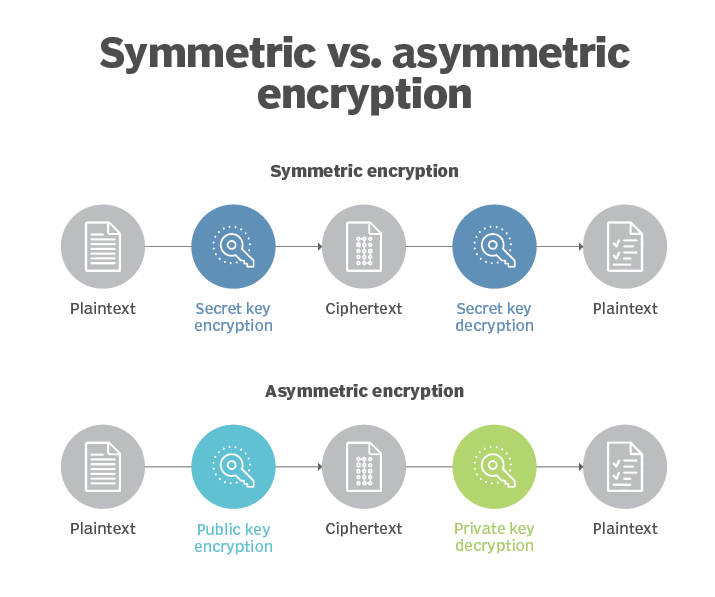
\includegraphics[width=.6\textwidth]{security-symmetric_vs_asymmetri_encryption.png}
\end{frame}

\subsection{Applicazioni}
\begin{frame}
    \frametitle{End-to-End Encryption}
    \framesubtitle{Applicazioni}

    \begin{itemize}
        \item \textbf{Comunicazioni sicure}: applicazioni di messaggistica e posta elettronica per mantenere private le conversazioni degli utenti;\pause
        \item \textbf{Gestione password}: a entrambi gli endpoint della comunicazione si trova lo stesso utente, l'unica persona munita di chiave;\pause
        \item \textbf{Data storage}: nei servizi di storage in cloud la E2EE protegge i dati degli utenti anche dall'accesso da parte dei fornitori del servizio in cloud.
    \end{itemize}

    \cite{IBM}
    
    \note{
        Alcuni sistemi, come ad esempio Lavabit e Hushmail, hanno in passato dichiarato di implementare la crittografia end-to-end nonostante ciò non fosse vero. \cite{lavabitAndHushmail} 

        Lavabit, servizio email in passato ritenuto sicuro e oggi non più attivo, nel 2014 consegnò al governo americano le chiavi che utilizzava per proteggere i dati dei propri utenti in occasione delle indagini sul caso Snowden. 
        La compagnia aveva in precedenza dichiarato che il proprio livello di sicurezza era tale che nemmeno gli amministratori avevano accesso al contenuto delle mail scambiate dai propri utenti. \cite{snowdenCase}, \cite{Snowden}

        Hushmail, altro email provider dichiarato sicuro, utilizzò le password dei propri utenti per decrittare le email e consegnarle al governo federale in \textit{plaintext}. \cite{hushmail}

        Altri sistemi, come per esempio Telegram, non implementano la crittografia end-to-end di default e sono pertanto stati criticati. 

        In modo particolare Telegram non la implementa né per le chat di gruppo né per i client desktop, oltre al fatto che utilizza il protocollo di crittografia non standard MTProto. \cite{telegramE2EE}
    }
\end{frame}
\subsection{Problematiche}

\begin{frame}
    \frametitle{End-to-End Encryption}
    \textbf{Problematiche}\newline

    La E2EE non garantisce di per sé né la sicurezza né la privacy, in quanto i dati trasmessi potrebbero essere protetti in modo poco sicuro sui dispositivi endpoint.\newline
    Tuttavia, l'implementazione della E2EE consente di applicare una protezione dei dati migliore della sola crittografia ``in transit''.\newline\pause

    Per molti sistemi di messaggistica i messaggi passano attraverso un intermediario che li conserva finché non vengono recuperati dal destinatario. Anche se protetti da crittografia, essi lo sono solamente in transito, quindi possono essere letti dai provider di servizi. 

    \cite{intransitEncryption}, \cite{IBM}

    \note{
        In questo modo è possibile monitorare il contenuto dei messaggi (per esempio in cerca di contenuti offensivi o pericolosi) ma si corre anche il rischio che utenti non autorizzati e/o malintenzionati aventi accesso allo storage dei messaggi possano fare un uso improprio dei contenuti.\newline

        Nella crittografia ``in transit'' è possibile o salvare direttamente i messaggi decrittati oppure salvare i dati crittografati e la chiave con cui decrittarli sullo stesso database.  
    }
\end{frame}

\begin{frame}
    \frametitle{End-to-End Encryption}
    Ulteriori problematiche: 
    \begin{itemize}
        \item \textbf{Endpoint security}: gli endpoint sono vulnerabili se non protetti adeguatamente\pause
        \item \textbf{Attacchi di tipo Man-in-the-Middle}: la conversazione può essere soggetta a \textit{eavesdropping}\pause
        \item \textbf{Backdoors}: si tratta di metodi per bypassare l'autenticazione standard o la protezione crittografica di un dispositivo. Se non volute, possono essere introdotte tramite attacchi cyber e poi sfruttate per violare la sicurezza del sistema
    \end{itemize}

    \cite{greenbergE2EE}, \cite{IBM}

    \note{
        \begin{itemize}
            \item Endpoint security: E2EE protegge i dati solo tra i due endpoint; ciò significa che i due endpoint possono essere soggetti ad attacchi;
            \item Attacchi MITM: anziché forzare la crittografia dei dati, ci si può aspettare un tentativo da parte di terzi malintenzionati di impersonare il destinatario durante. Essi possono, per esempio, impersonare il destinatario durante lo scambio di chiavi con il mittente, decifrare il messaggio inviato e poi inoltrarlo al vero destinatario senza farsi notare. Una soluzione per questo tipo di attacchi è introdurre un metodo di autenticazione (per es. certification authorities, web of trust, fingerprint numeriche o come QR code)
            \item Backdoors: nonostante le \textit{backdoors} non siano sempre implementate volutamente, esse possono essere introdotte grazie a \textit{cyber-attacks} e poi essere utilizzate per
            la negoziazione delle chiavi o per oltrepassare la protezione crittografica.
        \end{itemize}
    }
\end{frame}

\begin{frame}
    \frametitle{End-to-End Encryption} 
    \begin{itemize}
        \item \textbf{Complessità nel definire gli endpoint}: alcune implementazioni consentono di decodificare e ricodificare i dati lungo il percorso, quindi è necessario definire accuratamente gli estremi della trasmissione\pause
        \item \textbf{Privacy ``eccessiva''}: enti governativi non hanno modo di verificare la natura dei contenuti trasmessi dagli utenti, pertanto non sono in grado di prendere misure adeguate in caso di illeciti\pause
        \item \textbf{Metadati visibili}\pause
        \item Non vi è certezza che E2EE possa funzionare altrettanto bene con l'eventuale introduzione di \textit{quantum computer} che rendano la crittografia obsoleta
    \end{itemize}
    \cite{techTarget}
\end{frame}